\begin{frame}{Ethereum - Overview~\cite{bib:yellow}}
    \begin{itemize}
        \item Generalization of Bitcoin
        \item Support execution of \emph{quasi-}Turing Complete smart contracts
        \begin{itemize}
            \item Avoid abuse of network resources
            \item Each operation/opcode is associated with
            an amount of gas % $\implies$ termination guaranteed
            \item Gas price is determined per-transaction
        \end{itemize}
    \end{itemize}
\end{frame}

%% Ethereum Intro
\begin{frame}{Ethereum - World State~\cite{bib:yellow}}
    \begin{itemize}
    \item Save the world State ($\sigma$) explicitly
    \begin{itemize}
     \item Partial function from Addresses to Account States
     \item Externally owned account vs Contract Account
    \end{itemize}
    \end{itemize}

    \begin{figure}
        \begin{center}
            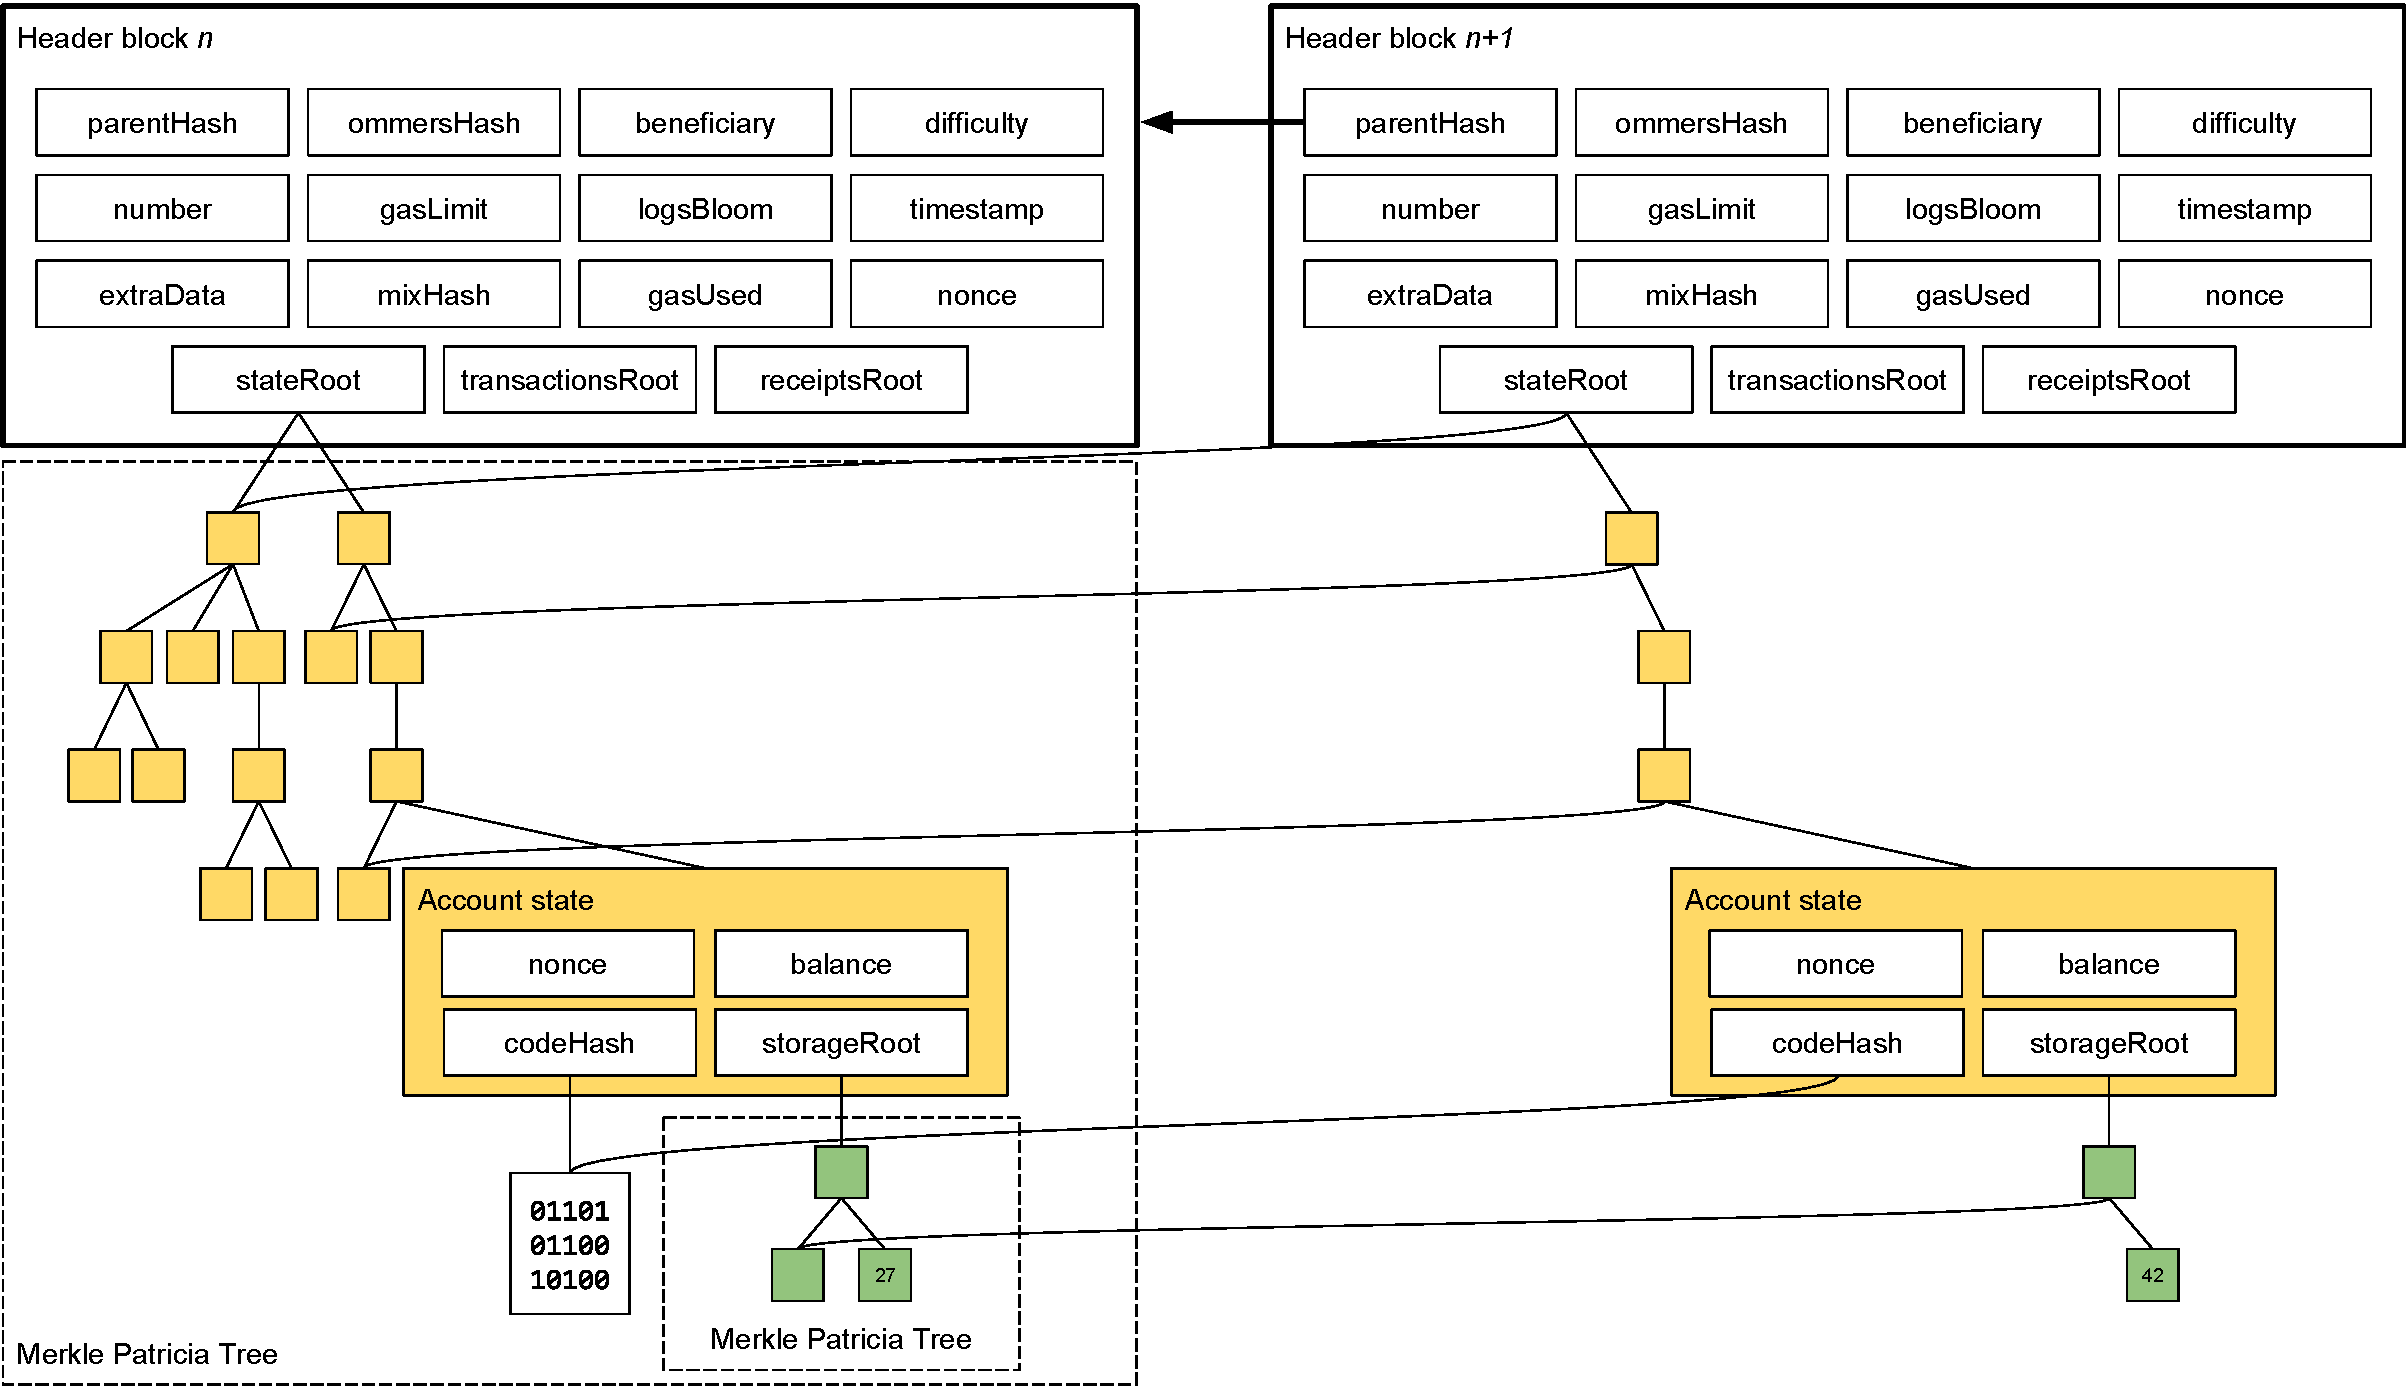
\includegraphics[width=0.92\textwidth]{./img/world-state}
        \end{center}
    \end{figure}
\end{frame}

\begin{frame}{Ethereum - Tx Execution~\cite{bib:yellow}}
%\begin{itemize}
%\item Transactions alter the state
%    \begin{itemize}
%    	\item Message Call
%        \item Contract Creation
%    \end{itemize}
%\end{itemize}
\begin{center}
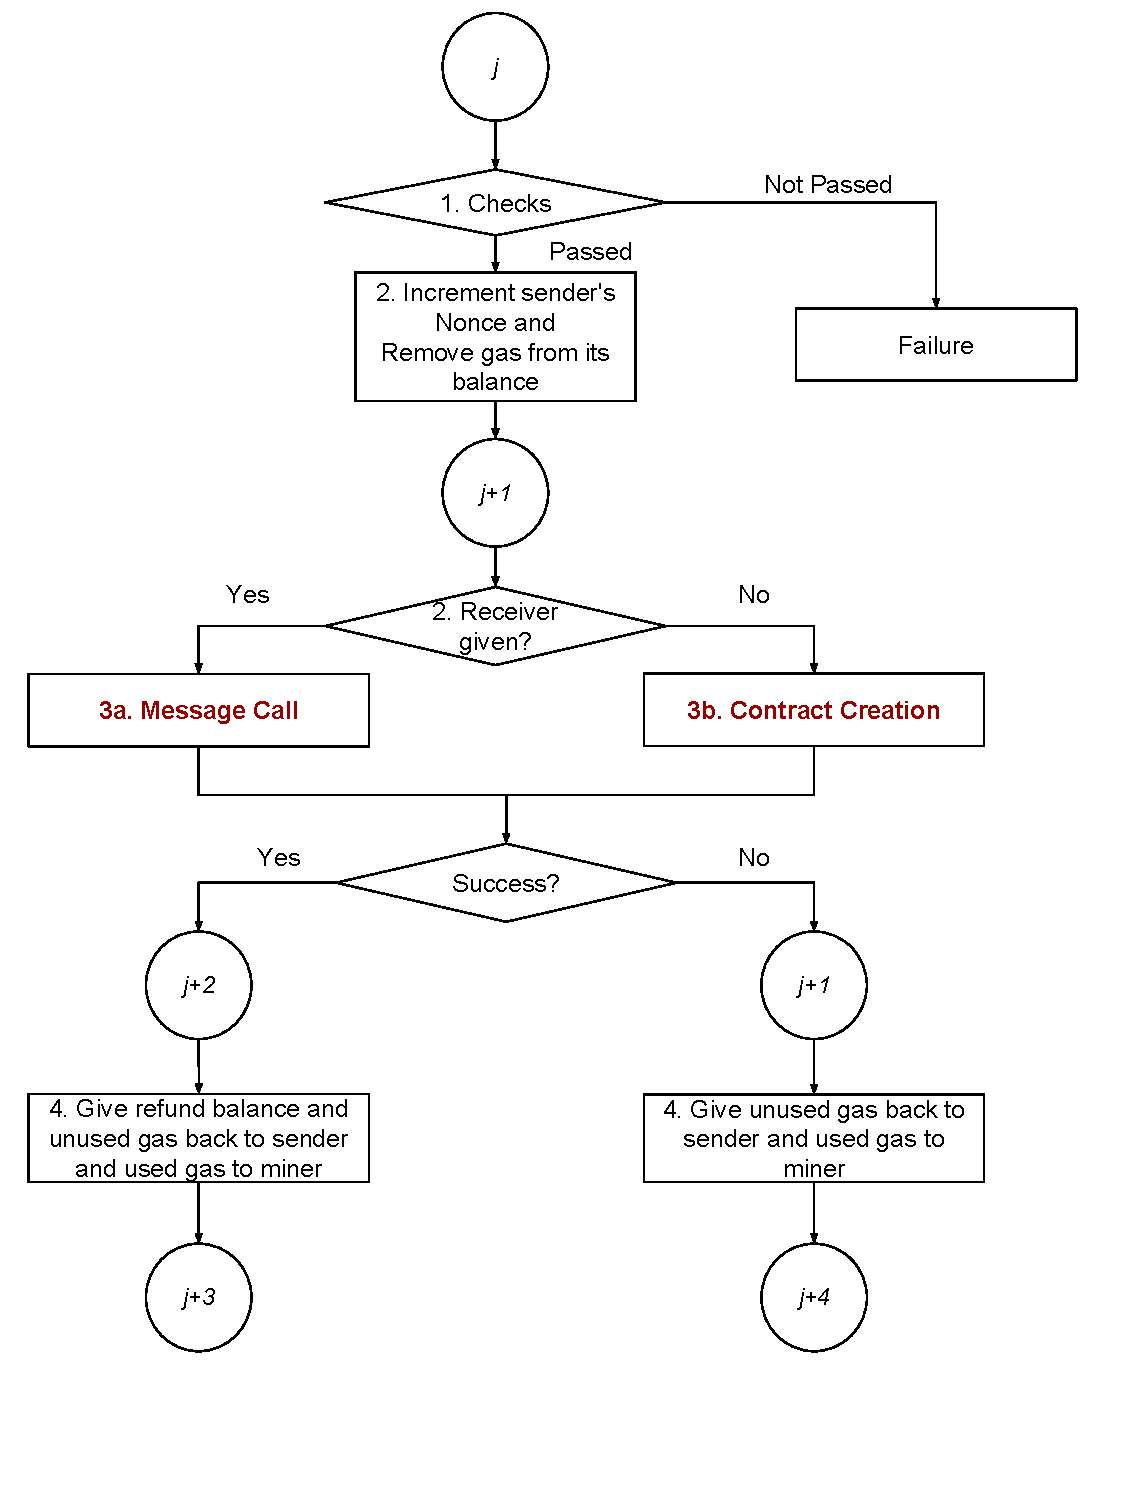
\includegraphics[height=0.85\textheight]{./img/transaction-execution}
\end{center}
\end{frame}


\begin{frame}{Execution Model - EVM~\cite{bib:yellow}}
\begin{center}
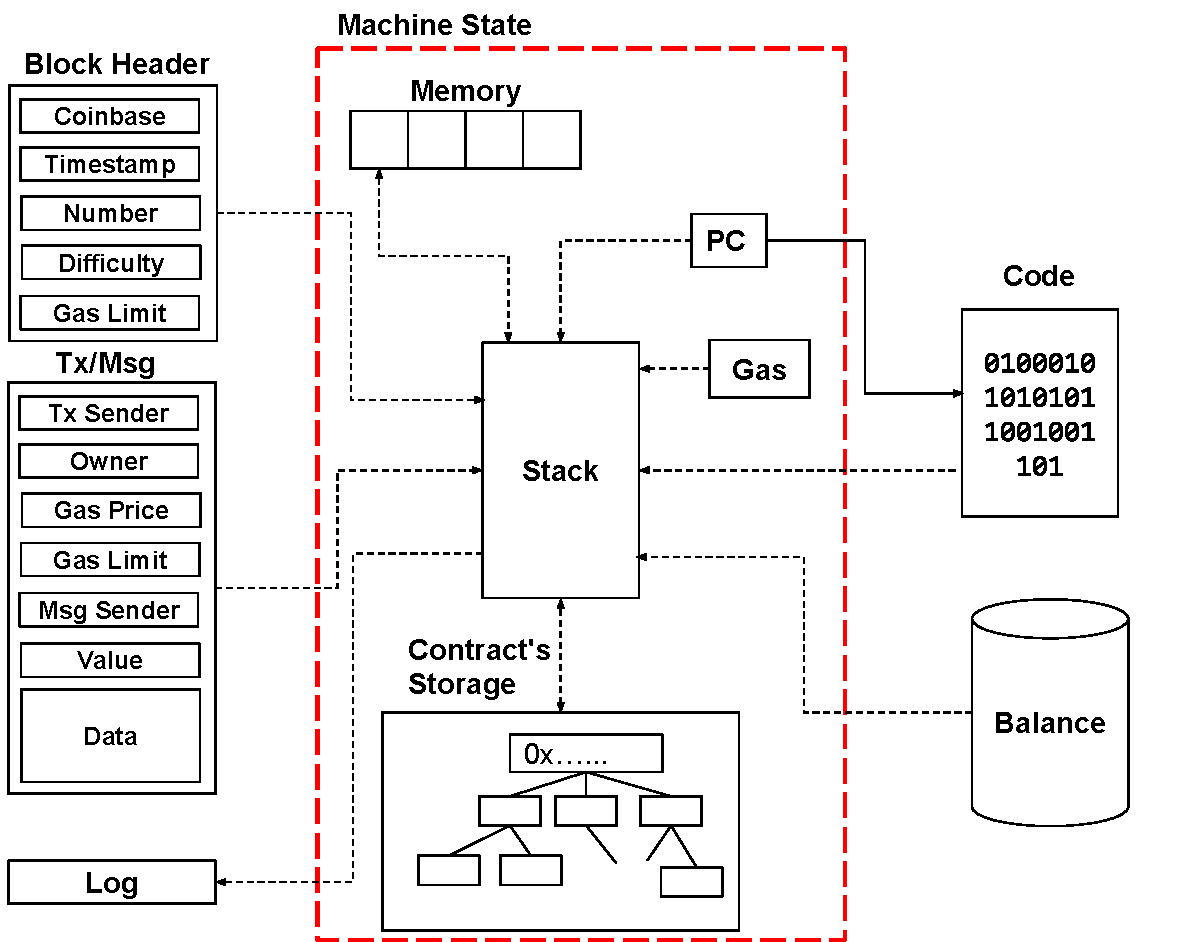
\includegraphics[width=0.8\textwidth]{./img/evm-overview}
\end{center}
\end{frame}

% EVM specifica nello yellow paper + molteplici formalizzazioni
% in letteratura



